\documentclass[secnumarabic,balancelastpage,amsmath,amssymb]{article}
%---------------------------------------ponemos los paquetes.--------------------------------------------%

\usepackage{amsmath}
\usepackage{amsthm}
\usepackage{amsfonts}
\usepackage{blindtext}
\usepackage{amssymb}
\usepackage{subfigure}
\usepackage{multicol}
\usepackage{graphicx}      % tools for importing graphics
\usepackage[utf8]{inputenc} %poner acentos
\usepackage[spanish]{babel} %titulos y descripciones en español
\usepackage[margin=2.0cm]{geometry} %modificar margenes del documento
%\cosas raras
\usepackage{bm}            % special bold-math package. usge: \bm{mathsymbol}
\usepackage[colorlinks=false]{hyperref} 
\usepackage{lscape}
\usepackage{titlesec} % Allows customization of titles
\renewcommand\thesection{\Roman{section}} % Roman numerals for the sections
\titleformat{\section}[block]{\large\scshape\centering}{\thesection.}{1em}{} % Change the look of the section titles
\titleformat{\subsection}[block]{\large}{\thesubsection.}{1em}{} % Change the look of the section titles
\providecommand{\abs}[1]{\lvert#1\rvert}
\providecommand{\norm}[1]{\lVert#1\rVert}


\newtheorem{theorem}{Theorem}[section]
\newtheorem{corollary}{Corollary}[theorem]
\newtheorem{lemma}[theorem]{Lemma}

\theoremstyle{remark}
\newtheorem*{remark}{Remark}

\theoremstyle{definition}
\newtheorem{definition}{Definición}[section]

\theoremstyle{prop}
\newtheorem{prop}{Proposición}[section]
\newtheorem{ejer}{Ejercicio}

%---------------------------------------inciamos el documento.--------------------------------------------%
\begin{document}


\title{\vspace{-15mm}\textbf{Resumen Semana 4}}
\author{\\ \emph{Equipo 19. Cálculo 3 - UNAM.}}


\maketitle
\section{Clase 16: 17/08/2020 }
\begin{definition}{Sea $f:X\rightarrow Y$ una función y $A\subset X$, Definimos y denotamos la imagen de A por:\\ 
$f(A)=\{ y \in Y :y=f(x)$ para alguna $x \in A\}$ }
\end{definition}

\begin{figure}[h!]
\centering.
\subfigure[]{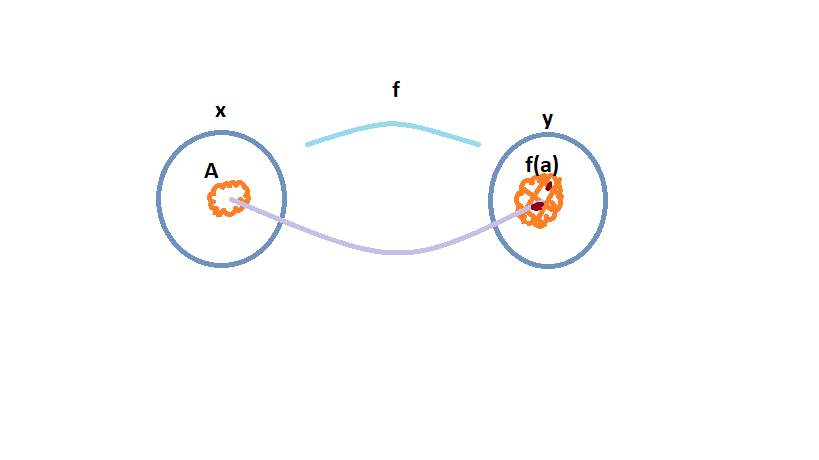
\includegraphics[width=80 mm]{1.png}}
\subfigure []{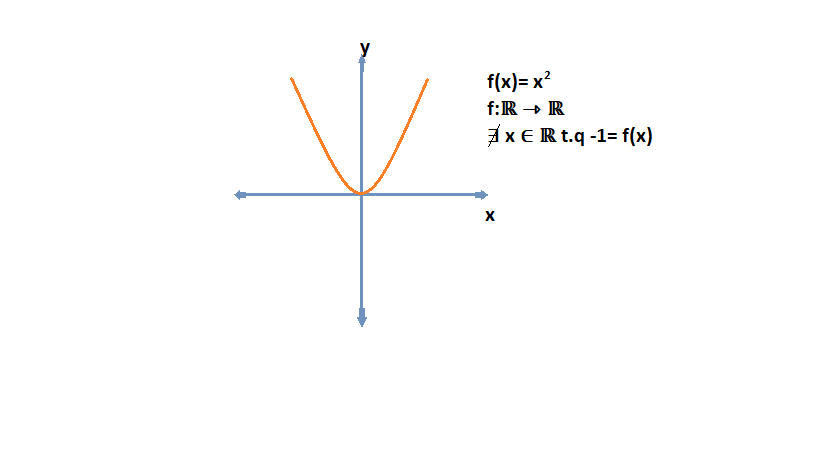
\includegraphics [width =80 mm]{imd1.png}}
\caption{Imagen directa}
\end{figure}





\begin{definition}{ Sea $f:X\rightarrow Y$ una función y $M \subset Y.$ Definimos y denotamos la imagen inversa de $M$ por: \\
$f^{-1}(M)= \{x \in X:f(x) \in M\}$}\end{definition}



\begin{figure}[h!]
\centering
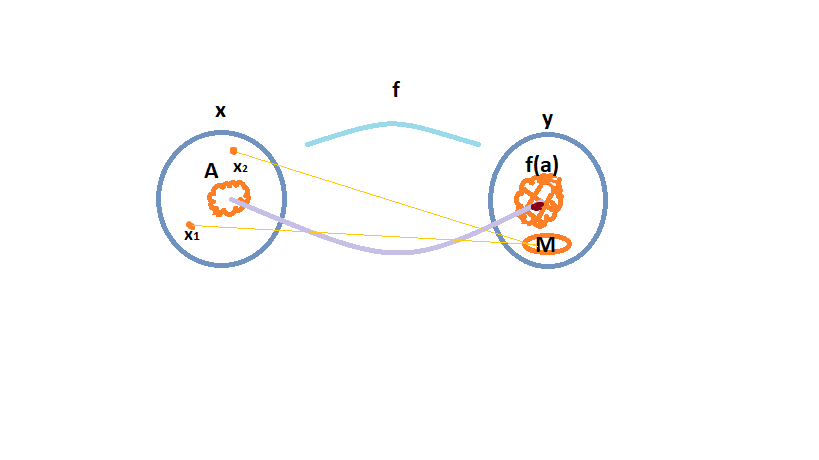
\includegraphics[width=0.4\textwidth]{imagen inversa.png}
\caption{Imagen Inversa.}
\label{fig:fig2.}
\end{figure}

\begin{prop} Sean $f:X\rightarrow Y$ una función y $A,B \subset X.$ Entonces.\\
\end{prop} 

\noindent 1.- $A \subset B \rightarrow f(A) \subset f(B) $\\
Dem: $y \in f(A) \Rightarrow y= f(x)$ p.a. $x \in A$, además $ A \subset B \Rightarrow x \in B \Rightarrow f(x) \in f(B)$ \\


2.- $ f(A \cup B)=f(A) \cup f(B) $\\
$\Rightarrow$ $f(A \cup B) \in f(A) \cup f(B)$\\
Sea $y \in f(A \cup B) \Rightarrow \exists x \in  A \cup B$ t.q. $y=f(x)$ \\
Si $x \in A \Rightarrow y=f(x) \in f(A) \Rightarrow y \in f(A) \cup f(B).$

$\Leftarrow$ Si $x \in B$.Análogamente al caso anterior $A \subset (A \cup B) \Rightarrow f(A) \subset f(A \cup B)$  Por prop. 1 y $f(B) \subset f(A \cup B) \Rightarrow f(A) \cup f(B) \subset$ \\

3.- $f(A \cap B) \subset f(A) \cap f(B)$\\
$A \cap B \subset A$ y $A \cap B \subset B$ Por prop. 1\\
$f(A \cap B) \subset f(A) y f(A \cap B) \subset f(B) $\\
$\Rightarrow$ $f(A \cap B) \subset f(A) \cap f(B)$\\

\begin{prop}{Sean $f:X\rightarrow Y $ donde $M \subset Y, f^{-1}(M)= \{x \in X:f(x) \in M\}$}
\end{prop}

\noindent 1.- $F \subset G \Rightarrow f^{-1}(F) \subset f^{-1}(G)$\\
Dem:$x \in f^{-1}(F) \Rightarrow f(x) \in F \subset G \Rightarrow f(x) \in G \Rightarrow x \in f^{-1}(G).$\\

2.- $f^{-1}(F \cup G)= f^{-1}(F) \cup f^{-1}(G)$\\
Dem: $\Rightarrow$ $x \in f^{-1}(F \cup G) \Rightarrow f(x) \in F \cup G \Rightarrow f(x) \in F \Rightarrow x \in f^{-1}(F) \Rightarrow x \in f^{-1}(F) \cup f^{-1}(G) $\\

$\Leftarrow$ $f^{-1}(F) \cup f^{-1}(G) \subset f^{-1}(F \cup G)$\\
$F \subset F \cup G \Rightarrow f^{-1}(F) \subset  f^{-1}(F \cup G)$ Por Prop.1 $\Rightarrow G \subset F \cup G \Rightarrow f^{-1}(G) \subset  f^{-1}(F \cup G) \Rightarrow f^{-1}(F) \cup  f^{-1}(G) \subset f^{-1}(F \cup G)$. \\

4.- $f^{-1}(F \setminus G)= f^{-1}(F)-f^{-1}(G)$\\
$\Rightarrow$ $x \in f^{-1}(F \setminus G) \Rightarrow f(x) \in (F \setminus G) \Rightarrow f(x) \subset F$ y $f(x) \not\in G \Rightarrow x \in f^{-1}(F)$ y $x \not\in f^{-1}(G) \Rightarrow x \in f^{-1}(F) \setminus  f^{-1}(G)$\\

$\Leftarrow$ $x \in f^{-1}(F) \setminus f^{-1} (G) \Rightarrow x \in F^{-1} (F)$ y $ x \not\in f^{-1} (G) \Rightarrow f(x) \in F$ y $ f(x) \not\in (G) \Rightarrow f(x) \in F \setminus G \Rightarrow x \in  f^{-1}$\\


\section{Clase 17: 18/08/2020}
Dudas.\\
\begin{ejer}
{2.- Calcular la ecuación parametrica de la recta que pasa por P(0,0,0) y es ortogonal a las rectas $L_{1}$ y $L_{2}$ cuyas ecuaciones parametricas están dadas por: }
\end{ejer}

\begin{multicols}{2}

 $\left \{
      \begin{array}{rcl}
          \ x=1+\lambda\\
          y=-2+4\lambda \\ 
         z=1+7\lambda 
      \end{array}
   \right . $\\  
   
   
 $\left \{
      \begin{array}{rcl}
          \ x=4+\mu\\
          y=1+2\mu \\ 
         z=-1+5\mu 
      \end{array}
   \right .$\\
     
\end{multicols} 

$\Rightarrow$ $L_{1}:(x,y,z)= \lambda \overline{u}+p_{1}$\\
$L_{2}:(x,y,z)= r\overline{v}+p_{2}$ $\Rightarrow$ $L:(x,y,z)= t\overline{w}$ $\Rightarrow$ $\overline{w}=\overline{u}\times \overline{v}$\\


\begin{multicols}{2}

$\left \{
      \begin{array}{rcl}
          \ x=1+\lambda\\
          y=-2+4\lambda \\ 
         z=1+7\lambda 
      \end{array}
   \right . $\\  
   
   $\left \{
      \begin{array}{rcl}
          \ x=4+\mu\\
          y=1+2+4\mu \\ 
         z=-1+5\mu 
      \end{array}
   \right . $\\   
   
  
   
   \end{multicols}
   
$(1,4,7)=\overline{u}$,  $p_{1}=(a,b,c)$ $\Rightarrow$ $(x,y,z)=\lambda(u_{1}, u_{2}, u_{3})+p $ \\

\begin{multicols}{2}
$\left \{
      \begin{array}{rcl}
          \ x=\lambda u_{1}+a\\
          y=\lambda u_{2}+b \\ 
         z=\lambda u_{3}+c
      \end{array}
   \right . $\\ 
   

   
 \end{multicols}   
 
 $L_{2} (1,2,5)=\overline{v}$ $\Rightarrow$ $\overline{w}=\overline{u}\times\overline{v}=(6,2,-2)$ $\Rightarrow$ $L:(x,y,z)=t(6,2,-2),t \in \mathbb {R}$
 $\Rightarrow$  $\left\{ 
      \begin{array}{rcl}
          \ x=6t\\
          y=2t\\ 
         z=-2t 
      \end{array}
   \right . $\\   
   
\begin{ejer}15.- Demuestre que el limite indicado no existe.

{\[
\lim_{(x,y) \to (0,0)} \frac{\sqrt[3]{x}y^{2}}{x+y^{3}}
   \]}
\end{ejer}
 Si evaluamos se indetermina entonces si $x=y$ $\Rightarrow$ $\frac{\sqrt[3]{x}x^{2}}{x+x^{3}}= \frac{x^{2/3}}{x+x^{3}}$ \\
Si $x=y^{3}$ $\Rightarrow$ $\frac{\sqrt[3]{y^{3}}y^{2}}{y^{3}+y^{3}}= \frac{y^{3}}{2y^{3}}=\frac{1}{2}$ Si $x=t^{6}$ y $y=-t$ $\Rightarrow$ $\frac{\sqrt[3]{t^{6}}t^{2}}{{t^{6}}-t^{3}}= \frac{t^{4}}{t^{6}-t^{3}}= \frac{t^{3}}{t^{3}}= \frac{t}{t^{3}-1}$ $\Rightarrow$ $t\rightarrow 0$ $\Rightarrow 0$\\

\subsection*{Superficie de nivel}
$f(x,y,z)= z^{2}+(\sqrt{x^{2}+y^{2}}-2)^{2}-1$
La gráfica vive en $\mathbb {R}^{4}$, no la podemos dibujar.\\
Superficie de nivel C.
$(x,y,z)/ z^{2}+(\sqrt{x^{2}+y^{2}-2)^{2}-1}=C$\\
$C=-1$    $C=0$     $C=1$ $\Rightarrow$ Si $x=0$ $(YZ)$ $\Rightarrow$ $\sqrt{y^{2}}= \abs{y}$ \\
$z^{2}+(\abs{y}-2)^{2}-1=C$\\
$z^{2}+(\abs{y}-2)^{2}=C+1>0$\\
 Si $y=0$ $(XZ)$ $\Rightarrow$ $z^{2}+(x-2)^{2}=C+1$\\
Si  $z=0$ $\Rightarrow$ $\sqrt{x^{2}+y^{2}-2)^{2}}=C+1$\\
$x^{2}+y^{2}-4\sqrt{x^{2}+y^{2}+4}=C+1$\\


\section{Clase 18: 19/08/2020}
\subsection*{(a) ($\cup_{\alpha \in I}A_{\alpha}) \cap B= \cup_{\alpha \in I}(A_{\alpha}\cap B)$}
$\Rightarrow$ $x \in (\cup_{\alpha \in I}A_{\alpha}) \cap B$\\
P.D. $x \in \cup_{\alpha \in I}(A_{\alpha}\cap B)$\\
$x \in \cup_{\alpha \in I} A_{\alpha}$ y $x \in B$ $\Rightarrow$ $x \in A_{\alpha 0}$ para algún, $\alpha_{0} \in I$ $\Rightarrow$ $x \in A_{\alpha 0} \cup B$ $\Rightarrow$ $\cap_{\alpha \in I}(\cup_{\alpha \in I} (A_{\alpha} \cap B).$\\
$\Leftarrow$ $x \in \cup_{\alpha \in I} (A_{\alpha}\cap B) \Rightarrow \exists \alpha_{0} \in I$ t.q. $x\in A_{\alpha 0}\cap B$
$\Rightarrow$ $x \in A_{\alpha 0}$ y $x\in B$ $\Rightarrow$ $x\in \cup_{\alpha \in I}$ y $x \in (\cup_{\alpha \in I} A_{\alpha}) \cap B$\\

$F= \{A_{\alpha}: \alpha \in I\}$
\subsection*{ (a) ($\cup_{\alpha \in I}A_{\alpha})^{c}= \cap_{\alpha \in I} A_{\alpha}^{c}$}

(b) ($\cap_{\alpha \in I}A_{\alpha})^{c}= \cup_{\alpha \in I} A_{\alpha}^{c}$\\

Demostración.\\
$\Rightarrow$ $x \in (\cap_{\alpha \in I} A_{\alpha})^{c}$ $\Rightarrow$ $x \notin A_{\alpha} \forall \alpha \in I$ 
$\Rightarrow$ Para cada $\alpha \in I, x \in A_{\alpha}^{c}$ $\Rightarrow$ 
$x \in \cup_{\alpha \in I} A_{\alpha}^{c}$\\
$\Leftarrow$ $x \in \cap_{\alpha \in I} A_{\alpha}^{c}$ $\Rightarrow$ $x \in A_{\alpha}^{c} \forall \alpha \in I$ $\Rightarrow$ $\notin A_{\alpha} \forall \alpha \in I$ $\Rightarrow$ $x \notin \cup_{\alpha \in I} A_{\alpha}$
$\Rightarrow$ $x \in (\cap_{\alpha \in I} A_{\alpha})^{c}$\\

\subsection*{5.- Demuestre que $\cap_{k=1}^{\infty} B_{\frac{1}{K}}(0)=\{0\}$}

\begin{figure}[h!]
\centering
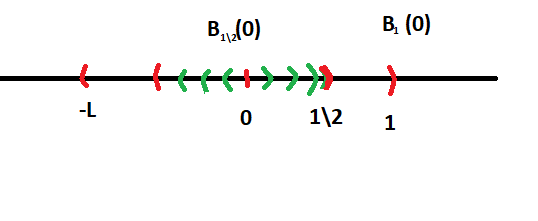
\includegraphics[width=0.4\textwidth]{5.PNG}
\label{fig:fig5.}
\end{figure}

$\cap_{k \in \mathbb {N} } (-\frac{1}{k},\frac{1}{k})= \{0\}$ si $\cap(\frac{1}{k},\frac{1}{k}) \not= \{0\}$ $\Rightarrow$ $\exists \epsilon >0$ t.q. $0<\epsilon< \frac{1}{k} \forall k \in \mathbb{N}$\\
$k< \frac{1}{\epsilon} \forall k \in \mathbb{N}!$\\
$\mathbb{N}$ no están acotados superiormente.\\

\subsection*{9.- Sea A= $\{ \frac{n}{n+1}: n \in \mathbb{N} \}$ Demuestra que A tiene solo un punto de acumulación. ¿Quien es la adherencia de A? y $F_{r}(A)$ y $A^{\circ}$}

\begin{figure}[h!]
\centering
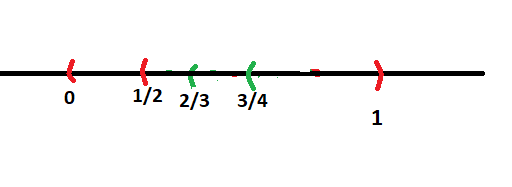
\includegraphics[width=0.4\textwidth]{9.PNG}
\label{fig:fig5.}
\end{figure}

$B_{r}(\frac{2}{3})|\frac{2}{3}) \cap A = \emptyset$\\

Af. $\forall$ $(B_{\epsilon}(1)| \{1\}) \cap A \not= \emptyset$\\
Sup. por el contrario que $\exists \epsilon>0$ t.q. $(B_{\epsilon}(1)| \{1\}) \cap A \not= \emptyset$ $\Rightarrow$ $\frac{n}{n+1} \leq 1-\epsilon  \forall n \in \mathbb{N}$\\
$\Rightarrow$ $n \leq (n+1)(1-\epsilon) \forall n \in \mathbb{N}$\\
$\Rightarrow$ $n \leq n-n \epsilon+1-\epsilon \forall n \in \mathbb{N}$ $\Rightarrow$ $n \leq \frac{1-\epsilon}{\epsilon} \forall n \in \mathbb{N} !$ \\

\subsection*{Composición de funciones continuas.}
Sean $f:U \subset \mathbb{R}^{n} \rightarrow \mathbb{R}^{m}$ y $g:V \subset \mathbb{R}^{m} \rightarrow \mathbb{R}^{p}$ donde $U$ es abierto en $\mathbb{R}^{n}$ y $V$ es abierto en $\mathbb{R}^{m}$\\
Si $f$ es continua en $x_{0}\in U$ entonces la función compuesta $g \circ f: U \subset \mathbb{R}^{p}$ es continua en $x_{0}$\\
Demostración. \\
Dado $\epsilon > 0$, por ser $g$ continua en $f(x_{0})$, existen $n>0$ tal que. $\norm{y-f(x_{0})} <n$ $\Rightarrow$ $\norm{g(y)-g(f(x)} < \epsilon$\\
Como $f$ es continua en $x_{0}$, existe $\delta > 0$ tal que\\
$\norm{x-x_{0}} < \delta$ $\Rightarrow$ $\norm{f(x)-f()x_{0}} < n$\\
De ambas aplicaciones concluimos que dado $\epsilon > 0$, existe $\delta> 0$ tal que\\
$\norm{x-x_{0}} < \delta$ $\Rightarrow$ $\norm{g(f(x_{0}))} < \epsilon$\\
Por lo tanto $g \circ f$ es continua en $x_{0}$

\section{Clase 19: 20/08/2020}
Dudas. \\
$f$ es una parametrizacion de una curva. $(\cos t, \sin t, 1-\sin t)$ $\Rightarrow$
$\left \{
      \begin{array}{rcl}
          \ x=\cos t\\
          y=\sin t \\ 
         z=1-\sin t 
      \end{array}
   \right . $  
Ecuación parametrica.\\
Sabemos $\cos ^{2}t+\sin^{2}t=1$ $\Rightarrow$ $x^{2}+y^{2}=1$ $\Rightarrow$ $z=1-y$ $\Rightarrow$ $0x+y+z-1=0$ $\Rightarrow$ $(0,1,1)= \overline{n}$\\

Ecuación de la Recta.\\
$(x,y,z)=t \overline{u}+ \overline{v}, t\in \mathbb{R}$\\
Param. $\gamma: \mathbb{R}\rightarrow\mathbb{R}^{3}$ $\Rightarrow$ $\gamma(t)=t\overline{u}+\overline{v}$ $\Rightarrow$ $t\rightarrow t\overline{u}+\overline{v}$

\begin{figure}[h!]
\centering
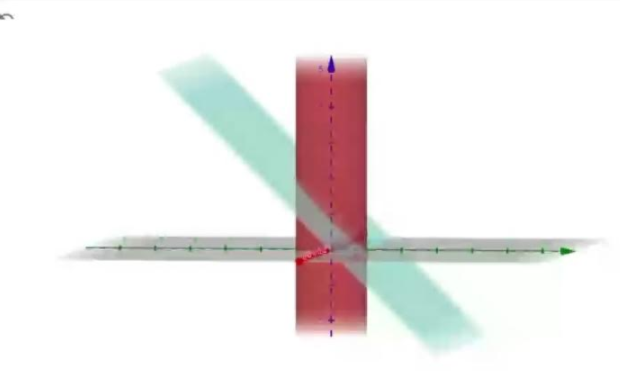
\includegraphics[width=0.4\textwidth]{cap1.PNG}
\label{fig:fig6.}
\end{figure}

$f: \mathbb{R}^{3} \rightarrow \mathbb{R}$ Función escalar \\
$f(x,y,z)=z^{2}+(\sqrt{x^{2}+y^{2}}-2)^{2}-1$\\
Encontrar la superficie de nivel para $C_{1}=-1$, $C_{2}=0$, $C_{3}=1$
$\Rightarrow$ $z^{2}+(\sqrt{x^{2}+y^{2}}-2)^{2}-1=-1$\\
$\Rightarrow$ $z^{2}+(\sqrt{x^{2}+y^{2}}-2)^{2}=0$ Superficie en $\mathbb{R}^{3}$ trazar $x=0$ plano (YZ) $\Rightarrow$ $z^{2}+(\abs{y}-2)^{2}=1$ $\Rightarrow$ $\sqrt{y^{2}}=\abs{y}$ $\Rightarrow$ $y=2$ o $y=-2$ $\Rightarrow$ Sol.$\{0,2,0\} , \{0,-2,0\}$ Con $y=0$ plano $(ZX)$ $z^{2}+(\abs{x}-2)^{2}=1$ circulo de radio $0$ $\Rightarrow$  Sol \{(2,0,0), (-2,0,0)\} \\
$z=0$ Plano (XY) $\Rightarrow$ $(\sqrt{x^{2}+y^{2}}-2)^{2}=0$ $\Rightarrow$ $\sqrt{x^{2}+y^{2}}-2=0$ $\Rightarrow$ $x^{2}+y^{2}=4$
$\Rightarrow$ $(\sqrt{x^{2}+y^{2}}-2)=1$ $\Rightarrow$ $x^{2}+y^{2}=9$ $\Rightarrow$ Circulo con radio $3$\\
$z^{2}+(\sqrt{x^{2}+y^{2}}-2)^{2}-1$ $\Rightarrow$ $z^{2}=-(\sqrt{x^{2}+y^{2}}-2)^{2}+1$ $\Rightarrow$ $z=\pm \sqrt{1-(\sqrt{x^{2}+y^{2}}-2)^{2}}$ Si $(x,y)$ cumple $1-(\sqrt{x^{2}+y^{2}}-2)^{2} \geq 0$ $\Rightarrow$ $1\geq(\sqrt{x^{2}+y^{2}}-2)^{2}$ Frontera $\Rightarrow$ $1=\sqrt{x^{2}+y^{2}}-2$ $\Rightarrow$ $3^{2}= x^{2}+y^{2}$ Es un circulo de radio $3$
\begin{figure}[h!]
\centering
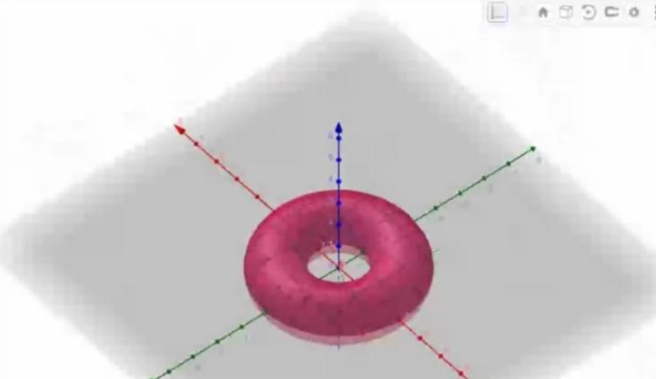
\includegraphics[width=0.4\textwidth]{Captura6.PNG}
\label{fig:fig7.}
\end{figure}

$\left \{
      \begin{array}{rcl}
          \ x=-1+2\lambda+3\mu\\
          y=4\lambda-\mu \\ 
         z=2-3\lambda+2\mu 
      \end{array}
   \right . $  
$\Rightarrow$ $2x-5y+z=0 :\pi_{2}$\\

$\pi :(x,y,z)= t\overline{u}+s\overline{v}+P$\\ $\overline{u}\times\overline{v}=\overline{n}= \Pi \cap \Pi$ \\
$<(x,y,z)-P,\overline{n}>=0$ Ecuación del plano\\
$\Rightarrow$ $\Pi_{1}=\lambda \overline{\alpha}+\mu\overline{\beta}+\overline{\gamma}=(x,y,z)$ $\Rightarrow$ $\lambda(2,4,-3)+\mu(3,\frac{-1}{\beta},2)+(-1,0,2)$
$\Rightarrow$ $\overline{\alpha}\times \overline{\beta}=\overline{n_{1}}$\\
$\Rightarrow$ $\Pi_{1}: <\overline{x}-\overline{\Gamma},\overline{n_{1}}=0$ Ecuación cartesiana.\\



\end{document}
 


